\documentclass[reprint, english,notitlepage]{revtex4-1}  % defines the basic parameters of the document
% if you want a single-column, remove reprint

% allows special characters (including æøå)
\usepackage[utf8]{inputenc}
\usepackage [norsk]{babel} %if you write norwegian
%\usepackage[english]{babel}  %if you write english


%% note that you may need to download some of these packages manually, it depends on your setup.
%% I recommend downloading TeXMaker, because it includes a large library of the most common packages.

\usepackage{physics,amssymb}  % mathematical symbols (physics imports amsmath)
\usepackage{graphicx}         % include graphics such as plots
\usepackage{xcolor}           % set colors
\usepackage{hyperref}         % automagic cross-referencing (this is GODLIKE)
\usepackage{tikz}             % draw figures manually
\usepackage{listings}         % display code
\usepackage{subfigure}        % imports a lot of cool and useful figure commands
\usepackage{verbatim}
\usepackage{adjustbox}

% defines the color of hyperref objects
% Blending two colors:  blue!80!black  =  80% blue and 20% black
\hypersetup{ % this is just my personal choice, feel free to change things
    colorlinks,
    linkcolor={red!50!black},
    citecolor={blue!50!black},
    urlcolor={blue!80!black}}

%% Defines the style of the programming listing
%% This is actually my personal template, go ahead and change stuff if you want
\lstset{ %
	inputpath=,
	backgroundcolor=\color{white!88!black},
	basicstyle={\ttfamily\scriptsize},
	commentstyle=\color{magenta},
	language=Python,
	morekeywords={True,False},
	tabsize=4,
	stringstyle=\color{green!55!black},
	frame=single,
	keywordstyle=\color{blue},
	showstringspaces=false,
	columns=fullflexible,
	keepspaces=true}

\begin{document}



\title{Ekstrasolare planeter 2}
\date{\today}
\author{Knadidatnr.: 15889}
\affiliation{Institute of Theoretical Astrophysics, University of Oslo}
\email{textme@astro.uio.no}


\newpage

\begin{abstract}
Jeg har gjort en simulasjon av et solsystem som består av en stjerne og syv planeter. Ved å regne på gravitasjonskreftene fra sola på planetene og fra de største planetene på sola, har jeg simulert flere omløp for legemene i sine baner om massesenteret i systemet. Man kan med ganske god tilnærming si at banene er sirkulære. Jeg har beregnet hvordan bevegelsen ville sett ut for en observatør som studerer systemet fra et annet solsystem, og ved å legge til støy i målingene klart å simulere måledata slik vi registrerer den fra fjerne stjerner i virkeligheten. Ved å studere Doppler-forskyvningen av spektrallinjer i lyset som når observatøren fra denne stjerna, er det mulig å påvise eksistensen til hvertfall én av planetene i bane rundt stjernen og gi et minste estimat for massen til den.

Jeg har også produsert fluksdata slik den ville sett ut for observatøren, der fluksen fra stjernen reduseres når planeter befinner seg mellom observatøren og stjernen. Med normal støy viste det seg å være umulig å finne ut noe om systemet ved å se på denne dataen. Det er derfor tydelig at det er svært mye informasjon om fjerne solsystemer vi ikke er i stand til å registrere.
\end{abstract}
\maketitle                                % creates the title, author, date & abstract



\section{Introduksjon}

Jeg skal i dette prosjektet utforske hvordan planetene i et solsystem påvirker stjernen de beveger seg rundt, og hvordan dette igjen påvirker hvordan lyset ser ut som når en observatør i et annet solsystem. Jeg skal studere et system som består av syv planeter og en stjerne med masse på ca. 87.9\% av solens masse. Jeg har tidligere, se \citep{paper1B}, simulert planetbanene i solsystemet uten å ta med gravitasjonskreftene som virker på sola. Ettersom massen til planetene er veldig liten i forhold til stjernens masse, kan dette være en grei tilnærming. Nå skal jeg gjøre samme simulasjon, men denne gangen også ta med gravitasjonskreftene som virker på sola fra de fire mest massive planetene i systemet.

Dette vil gjøre at stjernen beveger seg i bane rundt massesenteret til systemet. For en observatør et annet sted i verdensrommet vil det kanskje være mulig å se spor av denne bevegelsen ved å studere Doppler-forskyvningen av lyset som sendes ut av stjernen. Et eksempel på en slik analyse kan finnes i \citep{paper1C}. Man vil i så fall kun observere hastigheten i radiell retning sett fra observatørens planet. Jeg skal beregne den radielle hastigheten til stjernen i forhold til en tenkt observatør, og legge til støy i målingene for å simulere ekte data.

Jeg skal også simulere fluksdata som observatøren kunne mottatt fra stjernen. Etterhvert som planeter beveger seg foran stjernen, vil de blokkere en del av lyset slik at observatøren kan merke en redusert fluks. Dette kunne man brukt til å bestemme egenskaper ved planeten som går i bane rundt stjernen, igjen se \citep{paper1C}. Også i fluksdataen skal jeg legge til støy slik vi har for ekte måledata, og prøve å avgjøre om observatøren vil kunne observere at planetene beveger seg foran stjernen.

Å skjønne hvorfor dataen vi observerer fra fjerne stjerner ser ut som den gjør er viktig for å forstå hva vi kan lære av å studere den. I solsystemet jeg her studerer vet vi hvor mange planeter som finnes, og vi kjenner til mange av egenskapene ved dem. Ved å gjøre denne simulasjonen kan vi få et bilde på hvor mye vi faktisk observerer i fjerne solsystemer og hvor mye som kan finnes uten at vi er i stand til å oppdage det. Andre grunner til å simulere data kan være for å få tilgang til mer materiale som kan brukes til å utvikle eller teste metoder vi bruker til å behandle ekte data.



\section{Teori}

Newtons gravitasjonslov sier at gravitasjonskraften som virker på et legeme med masse $m_1$ fra
 et legeme med masse $m_2$ er
 \begin{equation}
   \label{eq:NGrav}
   \vec{F}_1 = \frac{G m_1 m_2}{r^2} \hat{\imath}_r
 \end{equation}
 der $\vec{F}_1$ er kraften som virker på legemet, $G$ er gravitasjonskonstanten, $r$ er avstanden mellom legemene og $\hat{\imath}_r$ er enhetsvektor som peker i retning fra $m_1$ mot $m_2$. Gravitasjonskraften på legeme $m_2$ er like stor men motsatt rettet: $\vec{F}_2 = -\vec{F}_1$.

Newtons 2. lov sier at akselerasjonen til et legeme er proporsjonal med nettokraften som virker
 på det:
 \begin{equation}
   \label{eq:N2}
   m \frac{\mathrm{d}^2 \vec{r}}{\mathrm{dt}^2} = \vec{F}_{\text{net}}
 \end{equation}
 Her er $m$ massen til legemet, $\vec{r}$ er posisjonen og $\vec{F}_{\text{net}}$ er nettokraften som virker på det.

Dersom gravitasjonskraften er den eneste kraften som virker på et legeme, får vi ved å kombinere
 likninger \ref{eq:NGrav} og \ref{eq:N2} at akselerasjonen til legemet med masse $m_1$ er
 \begin{equation}
   \label{eq:acc_planet}
   \frac{\mathrm{d}^2 \vec{r}_1}{\mathrm{dt}^2} = \frac{\vec{F}_1}{m_1} = \frac{G m_2}{r^3} \vec{r}
 \end{equation}
 Her er $m_2$ massen til det andre legemet, $\vec{r}$ er vektoren fra $m_1$ til $m_2$ og $r$ er avstanden mellom dem. Her har jeg brukt at $\hat{\imath}_r = \frac{\vec{r}}{r}$, der $r$ er lengden av vektor $\vec{r}$.

Har vi flere enn to legemer i et system, vil akselerasjonen til et av legeme være avhengig av
 gravitasjonskraften fra alle de andre legemene. Har vi bidrag fra flere legemer kan vi simpelthen summere bidragene fra hvert enkelt. Vi får at den totale akselerasjonen til legeme $i$ er
 \begin{equation}
   \label{eq:acc_star}
   \frac{\mathrm{d}^2 \vec{r}_i}{\mathrm{dt}^2} = \sum_{j \neq i} \frac{G m_j}{r_j^3} \vec{r_j}
 \end{equation}

Definisjonen for posisjonen til massesenteret til et system er \[\vec{R}_{\text{cm}} = \frac{\sum_i \vec{r}_i m_i}{\sum_i m_i} \] der vi summer over posisjonen og massene til alle legemene i systemet. $\vec{r}$ er posisjon og $m$ er masse. Posisjonen til et legeme i forhold til massesenteret er da gitt ved \[\vec{r}_{\text{cm}} = \vec{r} - \vec{R}_{\text{cm}}\] der $\vec{r}$ og $\vec{R}_{\text{cm}}$ er posisjonene til legemet og massesenteret i fohold til et annet referansepunkt. Ved å ta den tidsderiverte av disse likningene finner man at hastigheten til massesenteret er gitt ved: \[\vec{V}_{\text{cm}} = \frac{\sum_i \vec{v}_i m_i}{\sum_i m_i} \] Hastigheten til et legeme i forhold til massesenteret er gitt ved:
  \begin{equation}
    \label{eq:v_cm}
    \vec{v}_{\text{cm}} = \vec{v} - \vec{V}_{\text{cm}}
  \end{equation}





\section{Metode}

Jeg velger å simulere bevegelsen til de fire mest massive planetene i solsystemet. Jeg må ta med
 i beregningene gravitasjonskreftene fra hver av planetene på sola. For å bestemme planetenes baner tar jeg kun hensyn til gravitasjonskraften fra sola. Likning \ref{eq:acc_star} gir et uttrykk for akselerasjonen til stjernen. De ulike verdiene for j er indekser til hver av planetene. Likning \ref{eq:acc_planet} gir at akselerasjonen til hver av planetene er
 \begin{equation*}
   \frac{\mathrm{d}^2 \vec{r}_p}{\mathrm{dt}^2} = \frac{G M_{\star}}{r^3} \vec{r}
 \end{equation*}
 der $M_{\star}$ er massen til stjernen, $\vec{r}$ er vektoren fra planeten til stjernen og $r$ er avstanden mellom dem. Jeg løser differensiallikningene numerisk ved hjelp av Euler-Cromer. For en diskusjon av denne metoden, se \citep{paper1B}.

Det jeg egentlig er interessert i å finne er hastigheten til stjernen i forhold til
 massesenteret til solsystemet. Denne sammenhengen er gitt ved likning \ref{eq:v_cm}.

For å finne radiell hastighet til stjernen sett fra en observatør i et annet solsystem må jeg
 definere en siktlinje. Jeg velger å si at siktlinjen er langs y-aksen. Baneinklinasjonen er $i$, se figur \ref{fig:line_of_sight} i Appendix. Banefarten til stjernen langs siktlinjen er gitt ved \[v_{r, \text{orb}} = v_y \sin{i}\] der $v_y$ er banefarten til stjernen i forhold til massesenteret i solsystemet i y-retning og $i$ er baneinklinasjonen. ($v_y$ fordi siktlinjen er parallell med y-aksen). Den radielle hastigheten som observatøren registrerer blir da pekuliærhastigheten $v_{\text{pec}}$ pluss banefarten til stjernen langs siktlinjen:
 \begin{equation}
   \label{eq:v_r}
   v_r = v_{\text{pec}} + v_y \sin{i}
 \end{equation}
 Jeg velger verdier for $v_{\text{pec}}$ og $i$, og bruker verdiene for $v_y$ fra simulasjonen av
 bevegelsene i solsystemet.

Jeg legger til støy på verdiene av $v_r$ slik at den dataen man sitter igjen med likner på det vi observerer når vi studerer verdensrommet. Jeg regner med at støyen er normalfordelt med middelverdi 0 og et standardavvik som er en femtedel av maksverdien til $v_y$.

Jeg bruker ordet fluks til å beskrive hvor mye energi som når observatøren fra stjernen per tid. Jeg skal finne ut hvor mye fluksen reduseres når en planet passerer mellom stjerna og observatøren. Som et mål på dette bruker jeg relativ fluks; fluksen i ett tidssteg i forhold til den normale fluksen. Fluksen er proporsjonal med arealet som sender ut lys. Jeg antar at avstanden mellom stjerna og observatøren er så stor at når en planet beveger seg inn foran stjernen er dette arealet simpelthen stjernas tverrsnittareal minus planetens tversnittareal.

Jeg har allerede valgt siktlinje langs y-aksen. Det betyr at planetene kun skygger for stjerna når de befinner seg veldig nær y-aksen og samtidig under x-aksen. Nærmere bestemt når avstanden mellom massesenteret til planeten og massesenteret til stjerna er mindre enn radien til stjerna pluss radien til planeten. For enkelhets skyld tar jeg ikke hensyn til at mer og mer lys blir blokkert ettehvert som mer av planeten beveger seg inn foran stjerna. Jeg sier at når planeten er innenfor det området som er beskrevet over så er den relative fluksen redusert med \[\text{Reduksjon} = \frac{\text{Areal}_p}{\text{Areal}_{\star}} = \frac{\pi r_p^2}{\pi r_{\star}^2} = \left(\frac{r_p}{r_{\star}}\right)^2 \]
Her viser subindeks $p$ til planeten og $\star$ til stjerna, mens $r$ er radius.



\section{Resultater}

Ved å kjøre simuleringen med stjernens startposisjon i origo og initialfart 0 får jeg banene som
 er illustrert i figur \ref{fig:orbits}. Figur \ref{fig:rel_cm} viser stjernens posisjon og hastighet i forhold massesenteret i systemet under simulasjonen. Simulasjonen er kjørt med en million tidssteg på ca. 630s.

\begin{figure}
  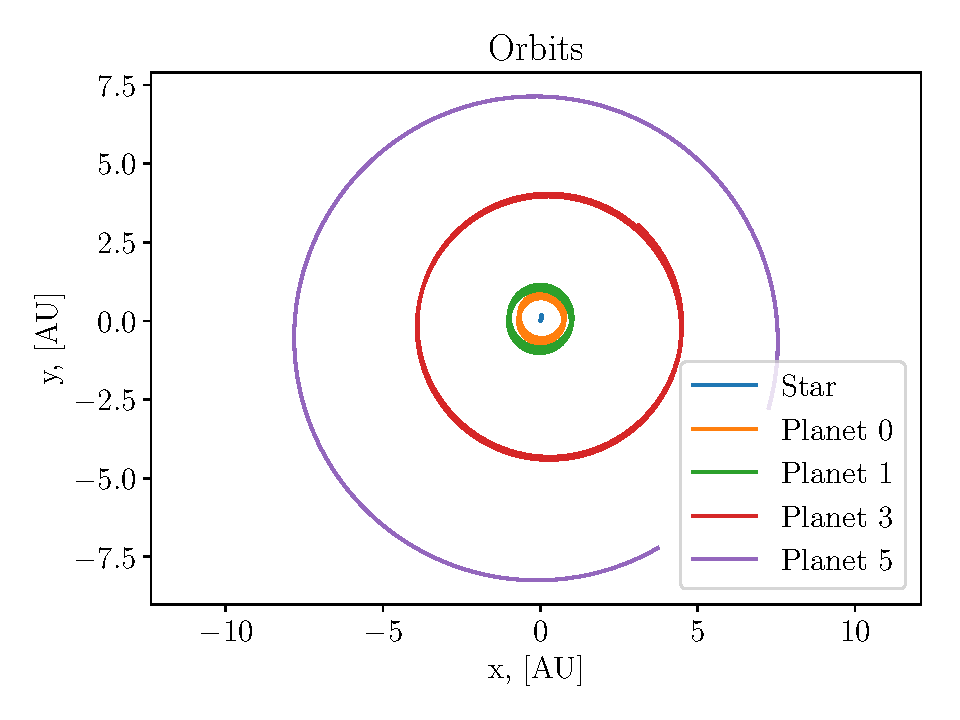
\includegraphics[width=\linewidth]{../output/plots/orbits.pdf}
  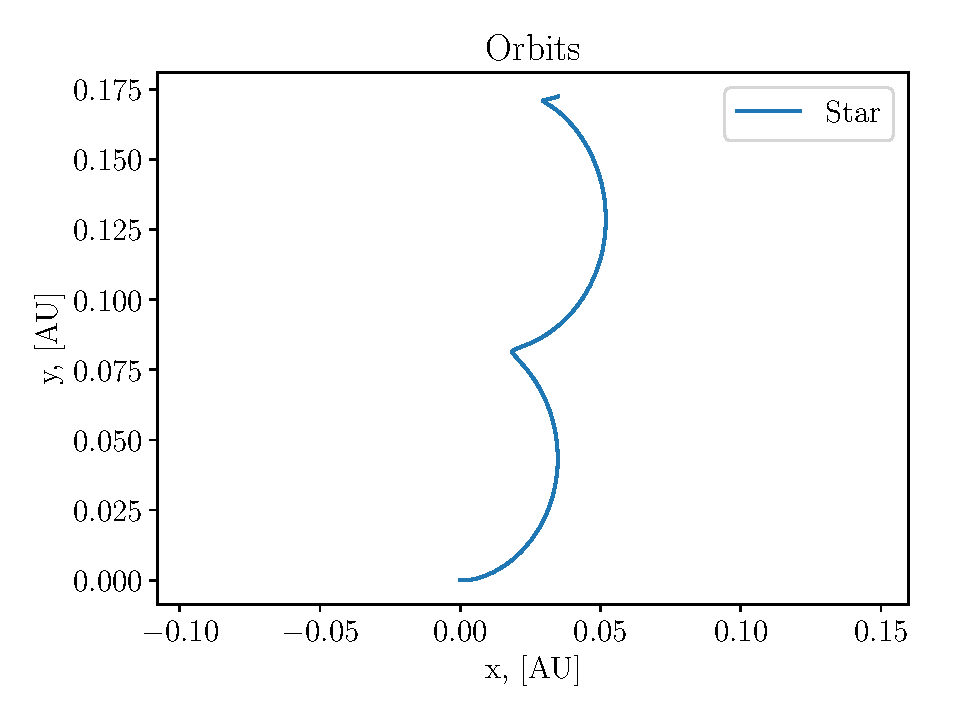
\includegraphics[width=\linewidth]{../output/plots/orbits_star.pdf}
  \caption{Den øverste figuren viser planetenes og stjernas baner. Under er den samme figuren, men fokusert på stjernen. Jeg bemerker at siden jeg setter initialfarten til stjernen lik 0, har vi som observatører hastighet ulik null i forhold til massesenteret til systemet. Dette er årsaken til at banene flytter seg oppover i bildet.}
  \label{fig:orbits}
\end{figure}

\begin{figure}
  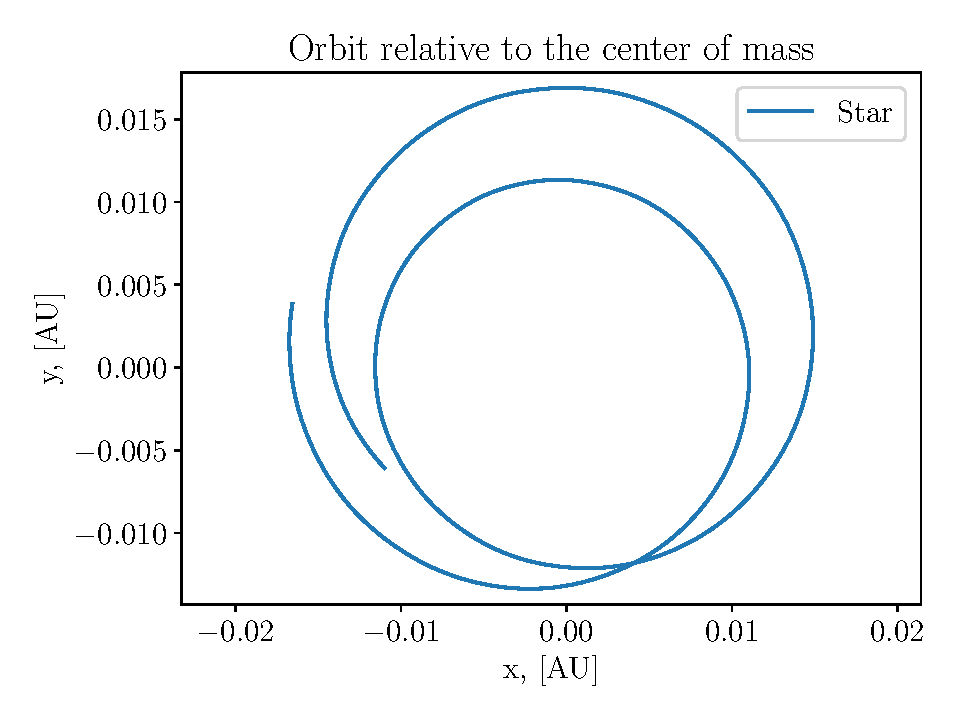
\includegraphics[width=\linewidth]{../output/plots/orbits_star_cm.pdf}
  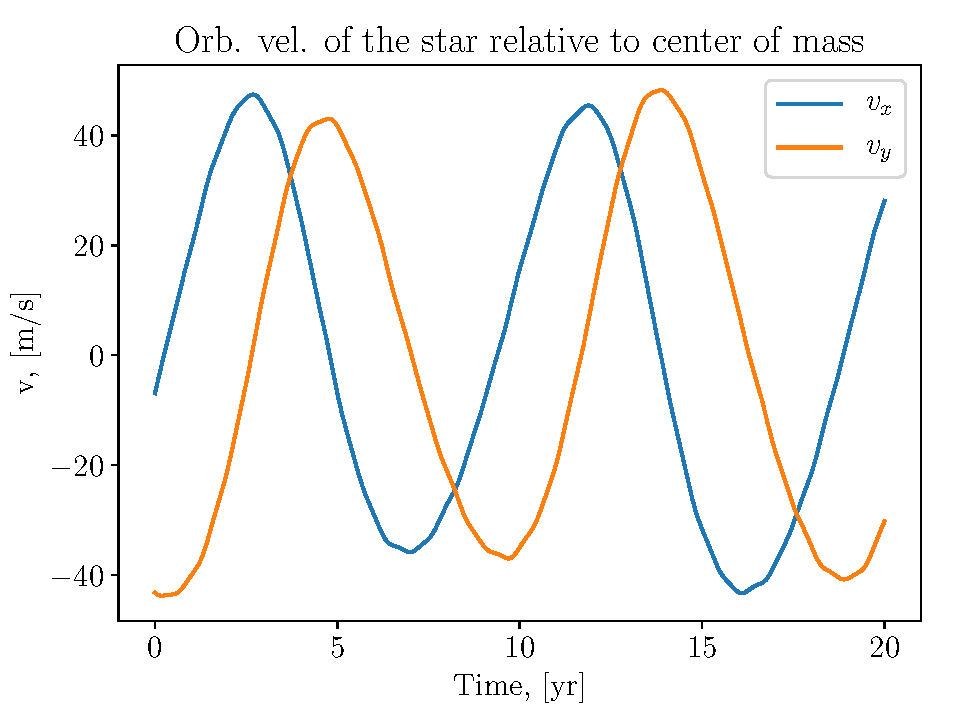
\includegraphics[width=\linewidth]{../output/plots/orbital_star_vel_cm.pdf}
  \caption{Den øverste figuren viser stjernens bane rundt massesenteret til systemet under simulasjonen. Figuren under viser stjernens hastighet i x-, og y-retning i forhold til massesenteret.}
  \label{fig:rel_cm}
\end{figure}

Figur \ref{fig:rad_vel} viser den radielle hastigheten slik en observatør ser det langs y-aksen.
 Inklinasjonsvinkelen $i$ er satt til $60^{\circ}$.
\begin{figure}
  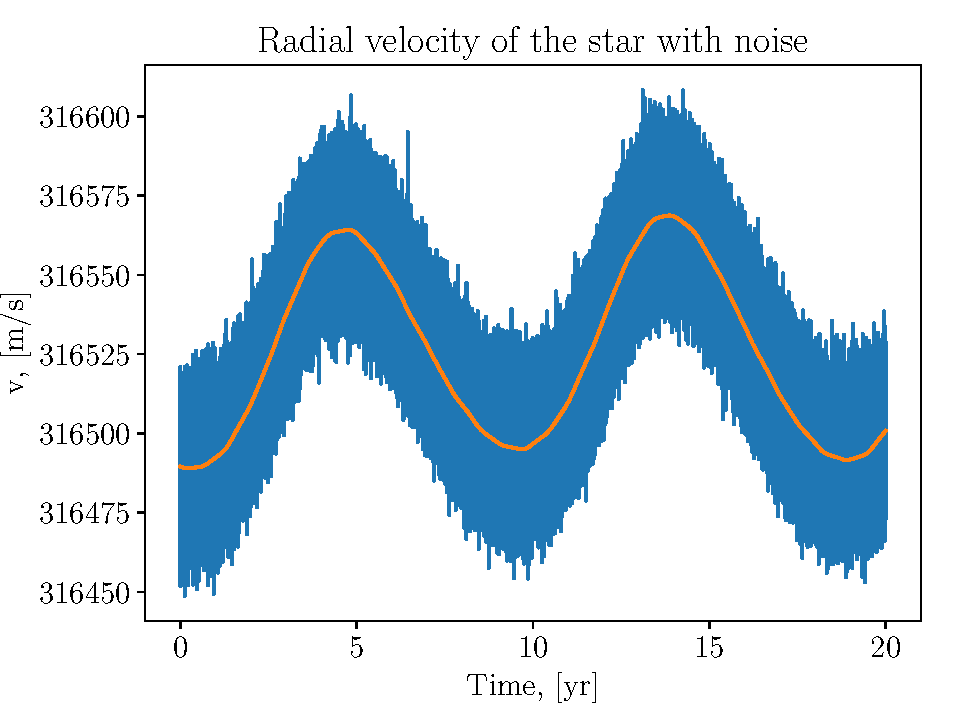
\includegraphics[width=\linewidth]{../output/plots/star_radial_vel.pdf}
  \caption{Radiell hastighet til stjernen med siktlinje langs y-aksen og inklinasjonsvinkel $i = 60^{\circ}$. Det blå er hastighetsverdiene med støy, den gule linjen viser hastigheten uten støy. Pekuliærhastighet er satt til 316 527m/s.}
  \label{fig:rad_vel}
\end{figure}

Figur \ref{fig:flux} viser den relative fluksen slik en observatør kan registrere det langs y-aksen. Den øverste figuren er uten støy, den nederste er med støy.
\begin{figure}
  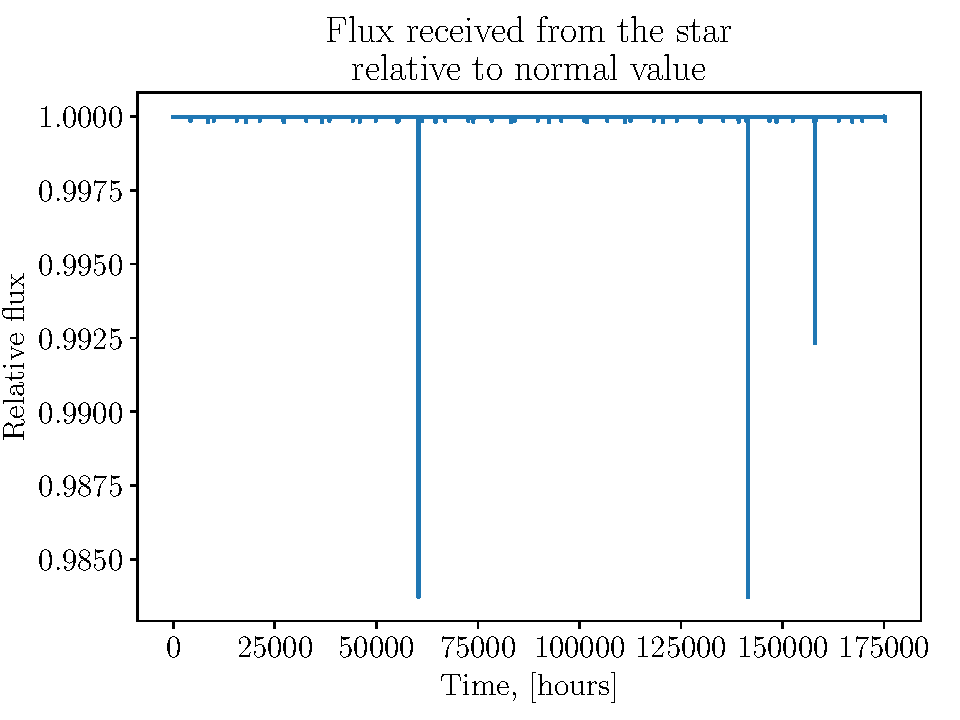
\includegraphics[width=\linewidth]{../output/plots/flux.pdf}
  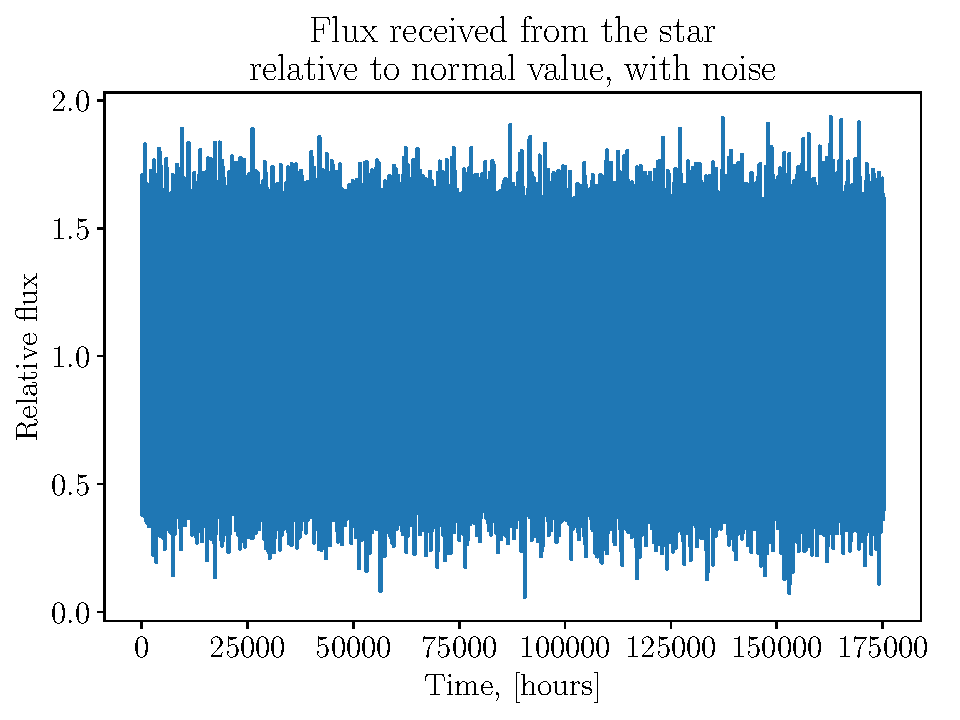
\includegraphics[width=\linewidth]{../output/plots/flux_noise.pdf}
  \caption{Den relative fluksen observert fra stjerna langs y-aksen. Den øverste figuren er uten støy, den nedre figuren er med normalfordelt støy med middelverdi 0 og standardavvik 0.2.}
  \label{fig:flux}
\end{figure}




\section{Diskusjon}

Jeg har beregnet planetbanene uten å ta med gravitasjonskreftene som virker mellom planetene, men simulasjonen vil likevel gi et ganske realistisk bilde på bevegelsene. Grunnen til dette er at tyngdekraften fra de andre planetene er forsvinnende liten i forhold til tyngdekraften fra stjernen. Massen til den største planeten i solsystemet er bare 0.3\% av stjernens masse, og de fleste andre planetene er flere størrelsesordener mindre enn det igjen.

Vi ser på den øverste illustrasjonen i figur \ref{fig:rel_cm} at stjernen beveger seg i bane rundt massesenteret i solsystemet. Man ser tydelig at banen ikke har form som en perfekt ellipse slik den ville hatt hvis vi bare hadde én planet i bane rundt den. Planetenes posisjon i forhold til stjernen varierer fra ett omløp til det neste slik at stjernen trekkes lenger unna eller nærmere massesenteret i noen omløp enn andre. Dette gjør at avstanden fra massesenteret til stjernen ikke er konstant, men varierer med tid og fra omløp til omløp. Banen er likevel ganske rund, og det er tydelig at vi ikke nødvendigvis gjør en stygg antakelse når vi regner med sirkulær stjernebanebane i studier av fjerne solsystemer (se for eksempel \citep{paper1C}).

Hastighetskurven til stjernen i forhold til massesenteret har omtrent form som en harmonisk svingning. Dette illustreres nederst i figur \ref{fig:rel_cm}. Hadde stjernens bane vært sirkulær med konstant banefart hadde vi hatt en perfekt harmonisk svingning. Det er tydelig at én planet har mye mer å si for stjernens bevegelse enn de andre. De store svingningene som er veldig tydelige i figuren skyldes gravitasjonskraften fra denne ene massive planeten. Man kan såvidt se små ujevnheter langs kurven som skyldes andre, mindre planeter. Disse små planetene ligger nærmere stjernen og har mindre omløpstid, og gravitasjonskraften fra dem gjør at vi får mange små svingninger langs kurven. Men hovedformen på kurven kommer fra én massiv planet. En observatør kan ved å studere denne kurven gi et estimat for den minste mulige massen til planeten$^{\citep{paper1C}}$.

Fra figur \ref{fig:rad_vel} ser vi at selv med støy i målingene er variasjonene i hastighet
 veldig tydelige. Variasjonene er riktignok veldig små i forhold til den totale hastigheten til stjerna i forhold til oss, men dette er ikke et problem. Vi kan observere endringer i en stjernes radielle hastighet på ned til 1m/s, se \citep{part1C}. Men med en mindre inklinasjonsvinkel ville sporene av stjernens bevegelse vært mindre tydelige, og ved $i = 0^{\circ}$ kunne vi ikke merket den i det hele tatt. Da hadde vi fått av likning \ref{eq:v_r} at $v_r = v_{\text{pec}}$ som er konstant. Størst variasjon ser vi med $i = 90^{\circ}$, da er det absolutt banefart i y-retning vi finner ved å trekke $v_{\text{pec}}$ fra den observerte hastigheten $v_r$.

Det er grunn til å tro at hastighetskurven ville sett veldig lik ut fra en annen synsvinkel. Det er bare én planet som har mye å si for stjernens bevegelse, og den har såpass mye mindre masse enn stjernen at stjernen beveger seg i en ganske sirkulær bane. Ved en perfekt sirkelbane ville vi ikke sett noen forskjell på hastighetskurven for forskjellige synsvinkler. Hadde vi derimot hatt en mer massiv planet, kunne banen til stjernen ha vært mer ellipseformet. Da er det ikke gitt at hastighetskurven ville blitt lik uansett synsvinkel, fordi banen kunne sett svært forskjellig ut langs for eksempel store halvakse i ellipsen i forhold til langs lille halvakse.

På figur \ref{fig:orbits_eclipse} er det markert når planetene er mellom observatøren og stjerna når siktlinjen er langs y-aksen. Figur \ref{fig:flux} viser hvordan fluksen varierer når planetene er i disse posisjonene. Vi ser tydelig på den øverste illustrasjonen av fluksen hva som skjer når planetene skygger for sola. De to nærmeste planetene har kortest omløpstid og minst radius. Vi ser derfor mange små reduksjoner av fluksen når disse planetene er foran stjerna. Den tredje planeten har størst radius og gir derfor størst reduksjon av fluksen. Dette skjer to ganger. Den femte planeten har størst omløpstid og passerer bare foran stjerna én gang. Den har litt mindre radius en planet nummer 3. På den nederste illustrasjonen av fluksen, der jeg har tatt med støy, er det helt umulig å se når de forskjellige planetene beveger seg foran sola. Avvikene som kommer av støyen er så mye større enn avvikene som kommer av planetenes bevegelser at det her ville vært helt umulig å observere planetene for en observatør langt unna. Dersom man var i stand til å registrere ved hjelp av fluksen når planeten beveget seg foran stjerna, kunne man, gitt tilstrekkelig presise målinger, regnet ut størrelsen til planeten og til og med størrelse og innhold i atmosfæren$^{\citep{paper1C}}$.

\begin{figure}
  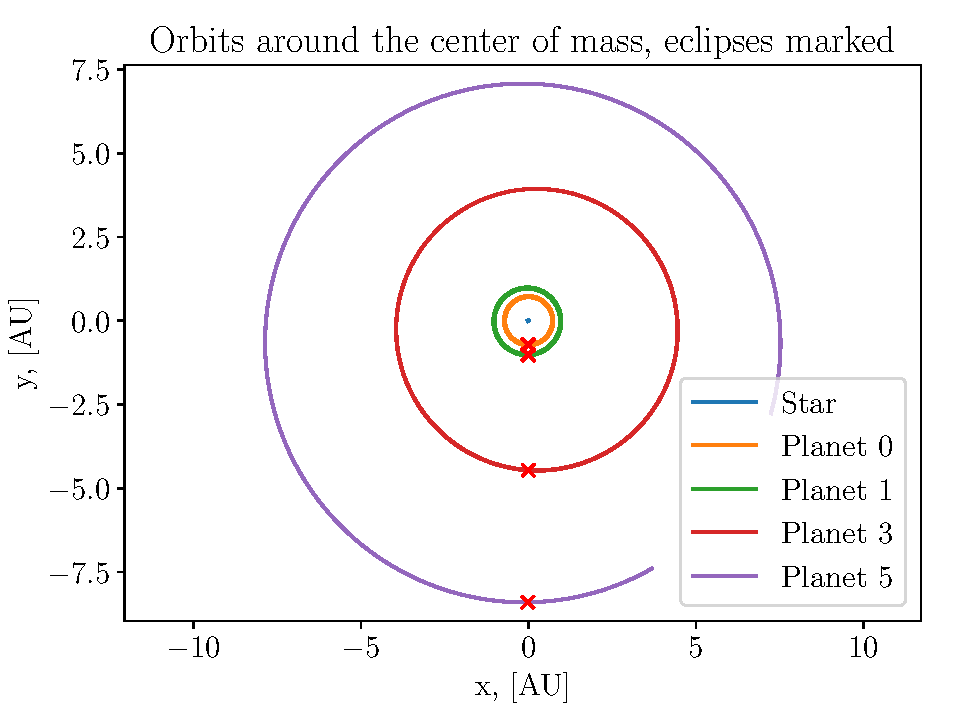
\includegraphics[width=\linewidth]{../output/plots/orbits_eclipse.pdf}
  \caption{Banene til planetene og stjerna i forhold til massesenteret i systemet. Røde kryss markerer alle punkter i banene der planetene befinner seg mellom observatøren og stjerna når siktlinja er langs y-aksen. Den observerte fluksen vil være redusert når planetene er i disse punktene.}
  \label{fig:orbits_eclipse}
\end{figure}



\section{Konklusjon}

Fra simulasjonen av bevegelsene i solsystemet ser man at både planeter og stjerna beveger seg i tilnærmet sirkulære baner rundt massesenteret i systemet. Det er litt variasjoner i radien i solas bane som kommer av at posisjonene som planetene trekker på stjerna fra endrer seg i løpet av simulasjonen. Vi kan likevel ofte med god tilnærming anta sirkelbane for fjerne stjerner når vi studerer dem, noe som gjør databehandlingen betydelig enklere.

Selv med støy er Doppler-forskyvning en anvendelig metode for å påvise planeter i bane rundt stjerner. Vi har måleutstyr som kan registrere svært små variasjoner i en stjernes bevegelse. Dette kan brukes til å finne estimater for den minste mulige massen planetene kan ha. Det er mye vanskeligere å finne presise tall på massen og størrelsen til planetene, og hvilke stoffer som finnes der. Det er ikke umulig, men det krever svært gode målinger og heldige forhold i solsystemet man studerer. Det er bemerkelsesverdig hvor mye man kan finne ut om fjerne solsystemer med relativt enkle metoder, men vi kan også konkludere med at det er svært mye informasjon vi absolutt ikke er i stand til å registrere med dagens teknologi og metoder.




\onecolumngrid
\vspace{1cm} % some extra space


\begin{thebibliography}{}
\bibitem[Hansen (2017)]{part1C} Hansen, F. K.,  2017, Forelesningsnotat 1C i kurset AST2000
\bibitem[15889 (2019)]{paper1B} 15889, Planetenes bevegelse i solsystemet
\bibitem[15889 (2019)]{paper1C} 15889, Ekstrasolare planeter


\end{thebibliography}


\section{Appendix}

\begin{figure}
  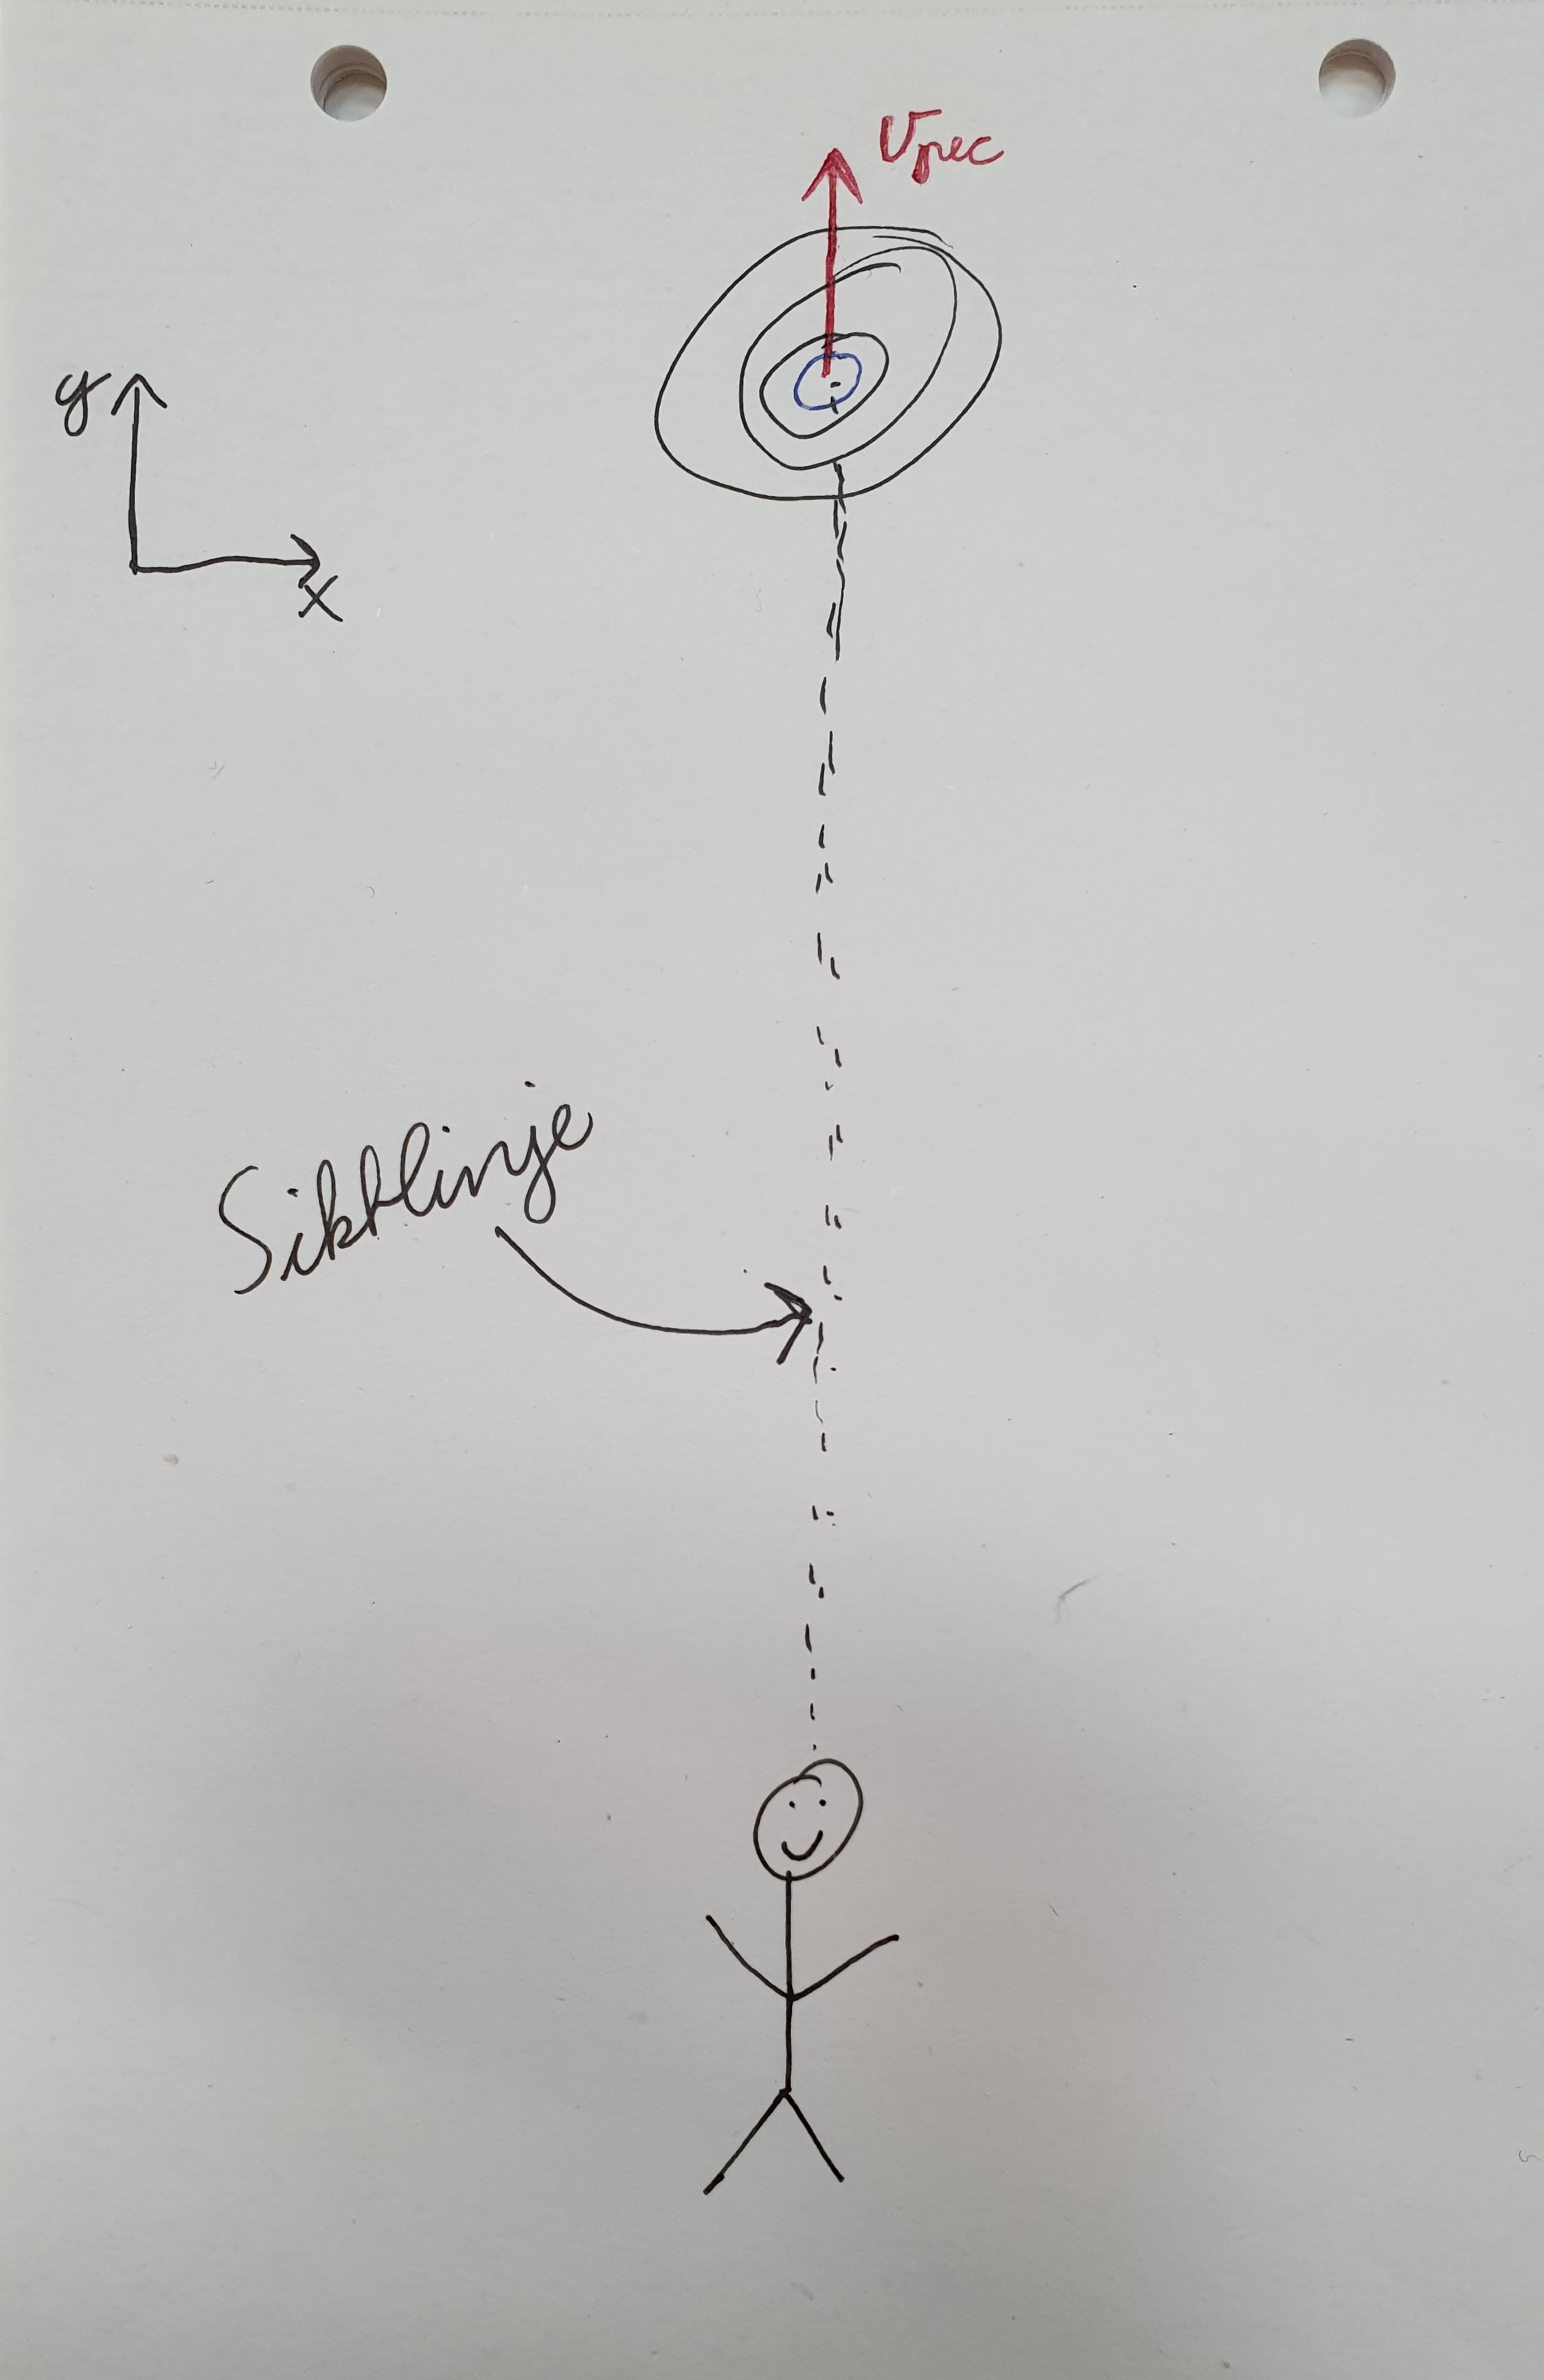
\includegraphics[width=10cm]{../output/line_of_sight2.jpg}
  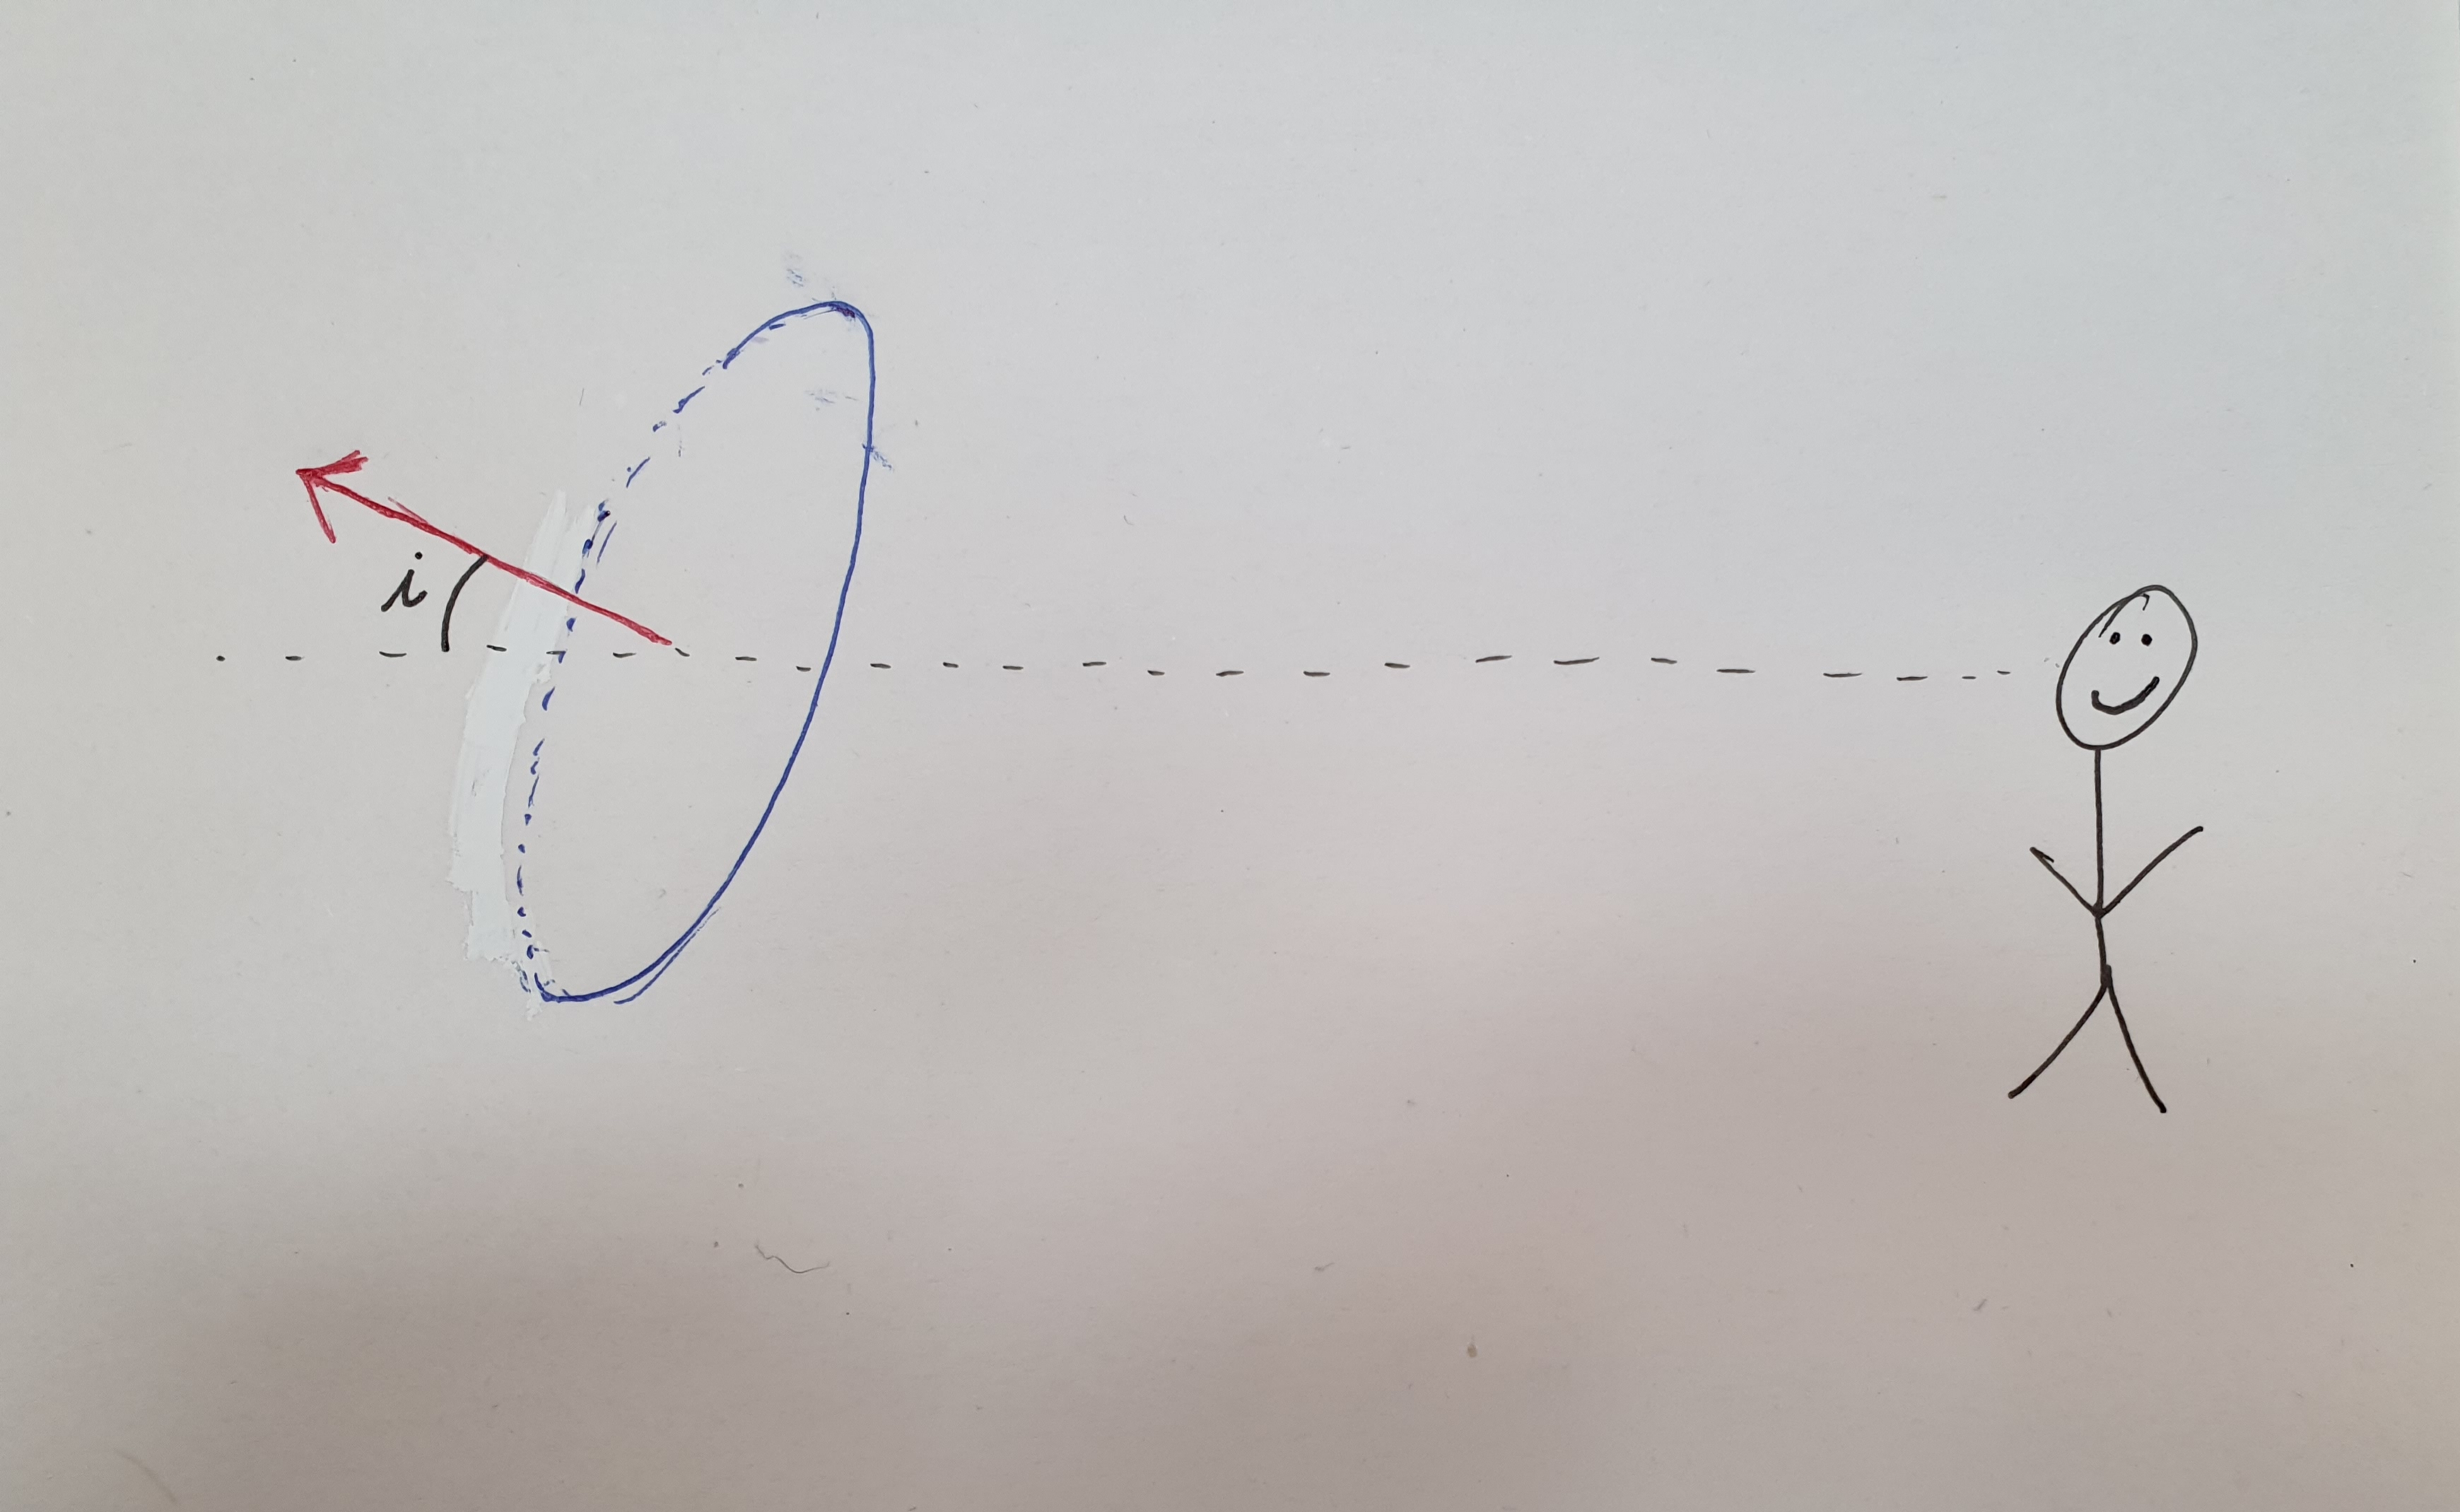
\includegraphics[width=10cm]{../output/line_of_sight1.jpg}
  \caption{Den øverste figuren viser at solsystemet beveger seg bort fra oss med en pekuliærhastighet $v_{\text{pec}}$, markert med rød pil. Siktlinjen er den stiplede linjen fra observatøren til systemet, den er parallell med y-aksen. Den nederste figuren viser baneinklinasjonen $i$. Med pekuliærhastigheten jeg har definert vil solsystemet bevege seg mot venstre i den nederste figuren.}
  \label{fig:line_of_sight}
\end{figure}


\end{document}
